
% This LaTeX was auto-generated from MATLAB code.
% To make changes, update the MATLAB code and republish this document.

\documentclass{article}
\usepackage{graphicx}
\usepackage{color}

\sloppy
\definecolor{lightgray}{gray}{0.5}
\setlength{\parindent}{0pt}

\begin{document}

    
    \begin{verbatim}
function varargout = gcs2017(varargin)
% GCS2017 MATLAB code for gcs2017.fig
%      GCS2017, by itself, creates a new GCS2017 or raises the existing
%      singleton*.
%      H = GCS2017 returns the handle to a new GCS2017 or the handle to
%      the existing singleton*.
%
%      GCS2017('CALLBACK',hObject,eventData,handles,...) calls the local
%      function named CALLBACK in GCS2017.M with the given input arguments.
%
%      GCS2017('Property','Value',...) creates a new GCS2017 or raises the
%      existing singleton*.  Starting from the left, property value pairs are
%      applied to the GUI before gcs2017_OpeningFcn gets called.  An
%      unrecognized property name or invalid value makes property application
%      stop.  All inputs are passed to gcs2017_OpeningFcn via varargin.
%
%      *See GUI Options on GUIDE's Tools menu.  Choose "GUI allows only one
%      instance to run (singleton)".
%
% See also: GUIDE, GUIDATA, GUIHANDLES

% Edit the above text to modify the response to help gcs2017

% Last Modified by GUIDE v2.5 22-Nov-2017 21:42:30

% Begin initialization code - DO NOT EDIT
gui_Singleton = 1;
gui_State = struct('gui_Name',       mfilename, ...
                   'gui_Singleton',  gui_Singleton, ...
                   'gui_OpeningFcn', @gcs2017_OpeningFcn, ...
                   'gui_OutputFcn',  @gcs2017_OutputFcn, ...
                   'gui_LayoutFcn',  [] , ...
                   'gui_Callback',   []);
if nargin && ischar(varargin{1})
    gui_State.gui_Callback = str2func(varargin{1});
end

if nargout
    [varargout{1:nargout}] = gui_mainfcn(gui_State, varargin{:});
else
    gui_mainfcn(gui_State, varargin{:});
end
% End initialization code - DO NOT EDIT

% --- Executes during object deletion, before destroying properties.
function figure1_DeleteFcn(hObject, eventdata, handles)
% hObject    handle to figure1 (see GCBO)
% eventdata  reserved - to be defined in a future version of MATLAB
% handles    structure with handles and user data (see GUIDATA)
StopTimerButtonfunc();

% --- Executes just before gcs2017 is made visible.
function gcs2017_OpeningFcn(hObject, eventdata, handles, varargin)
% This function has no output args, see OutputFcn.
% hObject    handle to figure
% eventdata  reserved - to be defined in a future version of MATLAB
% handles    structure with handles and user data (see GUIDATA)
% varargin   command line arguments to gcs2017 (see VARARGIN)

% Choose default command line output for gcs2017
handles.output = hObject;

% Update handles structure
guidata(hObject, handles);
axes (handles.logo);
imshow ('SenseAlert_2.JPG');

warning('off','all')
% lonAxis = [-79.3832 -79.3765];
% latAxis = [43.6565 43.6603];
% refLat = 43.658786;
% refLon = -79.380268;
% device_markerLoc = char(strcat({num2str(refLat,8)},{' '},{num2str(refLon,8)}));
% payload_markerLoc = char(strcat({num2str(refLat,8)},{' '},{num2str(refLon,8)}));
% axis(handles.axMap,[lonAxis, latAxis])
% plot_google_map('Axis',handles.axMap,'Marker',payload_markerLoc,'MapType','hybrid','AutoAxis',0)
%
global triggered
triggered = 0;

%CAnada Flag Logo addition
% axes (handles.CanadaFlag);
% imshow ('CanadaFlag.png');
%populate graph
%axes (handles.Graph1);
% UIWAIT makes gcs2017 wait for user response (see UIRESUME)
% uiwait(handles.figure1);
% Initial Arduino COMPORT Setup.
setCOMPort(handles);




% --- Outputs from this function are returned to the command line.
function varargout = gcs2017_OutputFcn(hObject, eventdata, handles)
% varargout  cell array for returning output args (see VARARGOUT);
% hObject    handle to figure
% eventdata  reserved - to be defined in a future version of MATLAB
% handles    structure with handles and user data (see GUIDATA)

% Get default command line output from handles structure
varargout{1} = handles.output;


% --- Executes on selection change in COMSelect.
function COMSelect_Callback(hObject, eventdata, handles)
% hObject    handle to COMSelect (see GCBO)
% eventdata  reserved - to be defined in a future version of MATLAB
% handles    structure with handles and user data (see GUIDATA)
setCOMPort(handles);

% Hints: contents = cellstr(get(hObject,'String')) returns COMSelect contents as cell array
%        contents{get(hObject,'Value')} returns selected item from COMSelect


% --- Executes during object creation, after setting all properties.
function COMSelect_CreateFcn(hObject, eventdata, handles)
% hObject    handle to COMSelect (see GCBO)
% eventdata  reserved - to be defined in a future version of MATLAB
% handles    empty - handles not created until after all CreateFcns called

% Hint: popupmenu controls usually have a white background on Windows.
%       See ISPC and COMPUTER.
if ispc && isequal(get(hObject,'BackgroundColor'), get(0,'defaultUicontrolBackgroundColor'))
    set(hObject,'BackgroundColor','white');
end


% --- Executes on button press in arduinoConnectButton.
function arduinoConnectButton_Callback(hObject, eventdata, handles)
% hObject    handle to arduinoConnectButton (see GCBO)
% eventdata  reserved - to be defined in a future version of MATLAB
% handles    structure with handles and user data (see GUIDATA)

global ard;
selectedPort = get(handles.COMSelect,'Value');
Portlist = get(handles.COMSelect,'String');
comport = Portlist{selectedPort};
% ard = connectFunction(comport, handles);

global ard2;
selectedPort2 = get(handles.COM2Select,'Value');
Portlist2 = get(handles.COM2Select,'String');
comport2 = Portlist2{selectedPort2};
% ard2 = connectFunction(comport2, handles);
[ard, ard2] = connectFunction(comport, comport2, handles);



% --- Executes during object creation, after setting all properties.
function uipanelGlider_CreateFcn(hObject, eventdata, handles)
% hObject    handle to uipanelGlider (see GCBO)
% eventdata  reserved - to be defined in a future version of MATLAB
% handles    empty - handles not created until after all CreateFcns called


% --- Executes during object deletion, before destroying properties.
function uitableDevice_DeleteFcn(hObject, eventdata, handles)
% hObject    handle to uitableDevice (see GCBO)
% eventdata  reserved - to be defined in a future version of MATLAB
% handles    structure with handles and user data (see GUIDATA)


% --- Executes when selected cell(s) is changed in uitableDevice.
function uitableDevice_CellSelectionCallback(hObject, eventdata, handles)
% hObject    handle to uitableDevice (see GCBO)
% eventdata  structure with the following fields (see MATLAB.UI.CONTROL.TABLE)
%	Indices: row and column indices of the cell(s) currently selecteds
% handles    structure with handles and user data (see GUIDATA)


% --- Executes during object creation, after setting all properties.
function uitableDevice_CreateFcn(hObject, eventdata, handles)
% hObject    handle to uitableDevice (see GCBO)
% eventdata  reserved - to be defined in a future version of MATLAB
% handles    empty - handles not created until after all CreateFcns called


% --- Executes on selection change in graphxAxis.
function graphxAxis_Callback(hObject, eventdata, handles)
% hObject    handle to graphxAxis (see GCBO)
% eventdata  reserved - to be defined in a future version of MATLAB
% handles    structure with handles and user data (see GUIDATA)

% Hints: contents = cellstr(get(hObject,'String')) returns graphxAxis contents as cell array
%        contents{get(hObject,'Value')} returns selected item from graphxAxis


% --- Executes during object creation, after setting all properties.
function graphxAxis_CreateFcn(hObject, eventdata, handles)
% hObject    handle to graphxAxis (see GCBO)
% eventdata  reserved - to be defined in a future version of MATLAB
% handles    empty - handles not created until after all CreateFcns called

% Hint: popupmenu controls usually have a white background on Windows.
%       See ISPC and COMPUTER.
if ispc && isequal(get(hObject,'BackgroundColor'), get(0,'defaultUicontrolBackgroundColor'))
    set(hObject,'BackgroundColor','white');
end


% --- Executes on selection change in graphyAxis.
function graphyAxis_Callback(hObject, eventdata, handles)
% hObject    handle to graphyAxis (see GCBO)
% eventdata  reserved - to be defined in a future version of MATLAB
% handles    structure with handles and user data (see GUIDATA)

% Hints: contents = cellstr(get(hObject,'String')) returns graphyAxis contents as cell array
%        contents{get(hObject,'Value')} returns selected item from graphyAxis


% --- Executes during object creation, after setting all properties.
function graphyAxis_CreateFcn(hObject, eventdata, handles)
% hObject    handle to graphyAxis (see GCBO)
% eventdata  reserved - to be defined in a future version of MATLAB
% handles    empty - handles not created until after all CreateFcns called

% Hint: popupmenu controls usually have a white background on Windows.
%       See ISPC and COMPUTER.
if ispc && isequal(get(hObject,'BackgroundColor'), get(0,'defaultUicontrolBackgroundColor'))
    set(hObject,'BackgroundColor','white');
end


% --- Executes during object creation, after setting all properties.
function logo_CreateFcn(hObject, eventdata, handles)
% hObject    handle to logo (see GCBO)
% eventdata  reserved - to be defined in a future version of MATLAB
% handles    empty - handles not created until after all CreateFcns called

% Hint: place code in OpeningFcn to populate logo



% --- Executes on button press in stopTimer.
function stopTimer_Callback(hObject, eventdata, handles)
% hObject    handle to stopTimer (see GCBO)
% eventdata  reserved - to be defined in a future version of MATLAB
% handles    structure with handles and user data (see GUIDATA)
stopTimerFunction();


% --- Executes on button press in startBurn.
function startBurn_Callback(hObject, eventdata, handles)
% hObject    handle to startBurn (see GCBO)
% eventdata  reserved - to be defined in a future version of MATLAB
% handles    structure with handles and user data (see GUIDATA)
global ard;
fprintf('%c\n', 'B');



% --- Executes on button press in deploymentButton.
function deploymentButton_Callback(hObject, eventdata, handles)
% hObject    handle to deploymentButton (see GCBO)
% eventdata  reserved - to be defined in a future version of MATLAB
% handles    structure with handles and user data (see GUIDATA)
global matrix;





% --- Executes on selection change in COM2Select.
function COM2Select_Callback(hObject, eventdata, handles)
% hObject    handle to COM2Select (see GCBO)
% eventdata  reserved - to be defined in a future version of MATLAB
% handles    structure with handles and user data (see GUIDATA)

% Hints: contents = cellstr(get(hObject,'String')) returns COM2Select contents as cell array
%        contents{get(hObject,'Value')} returns selected item from COM2Select


% --- Executes during object creation, after setting all properties.
function COM2Select_CreateFcn(hObject, eventdata, handles)
% hObject    handle to COM2Select (see GCBO)
% eventdata  reserved - to be defined in a future version of MATLAB
% handles    empty - handles not created until after all CreateFcns called

% Hint: popupmenu controls usually have a white background on Windows.
%       See ISPC and COMPUTER.
if ispc && isequal(get(hObject,'BackgroundColor'), get(0,'defaultUicontrolBackgroundColor'))
    set(hObject,'BackgroundColor','white');
end


% --- Executes during object creation, after setting all properties.
function Graph1_CreateFcn(hObject, eventdata, handles)
% hObject    handle to Graph1 (see GCBO)
% eventdata  reserved - to be defined in a future version of MATLAB
% handles    empty - handles not created until after all CreateFcns called

% Hint: place code in OpeningFcn to populate Graph1
handles.Graph1=hObject; % tag for this axis, which I call axesX in this example
guidata(hObject, handles); % update the handles structure for the gui


% --- Executes during object creation, after setting all properties.
function uitablePayload_CreateFcn(hObject, eventdata, handles)
% hObject    handle to uitablePayload (see GCBO)
% eventdata  reserved - to be defined in a future version of MATLAB
% handles    empty - handles not created until after all CreateFcns called


% --- Executes during object creation, after setting all properties.
function figure1_CreateFcn(hObject, eventdata, handles)
% hObject    handle to figure1 (see GCBO)
% eventdata  reserved - to be defined in a future version of MATLAB
% handles    empty - handles not created until after all CreateFcns called
% This creates the 'background' axes
% ha = axes('units','normalized', ...
%             'position',[0 0 1 1]);
% % Move the background axes to the bottom
% uistack(ha,'bottom');
% % Load in a background image and display it using the correct colors
% % The image used below, is in the Image Processing Toolbox.  If you do not have %access to this toolbox, you can use another image file instead.
% I=imread('background.jpg');
% hi = imagesc(I)
% colormap gray
% % Turn the handlevisibility off so that we don't inadvertently plot into the axes again
% % Also, make the axes invisible
% set(ha,'handlevisibility','off', ...
%             'visible','off')


% --- Executes during object creation, after setting all properties.
function property_CreateFcn(hObject, eventdata, handles)
% hObject    handle to property (see GCBO)
% eventdata  reserved - to be defined in a future version of MATLAB
% handles    empty - handles not created until after all CreateFcns called
%set(handles.property,'BackgroundColor','none')


% --- Executes when property is resized.
function property_SizeChangedFcn(hObject, eventdata, handles)
% hObject    handle to property (see GCBO)
% eventdata  reserved - to be defined in a future version of MATLAB
% handles    structure with handles and user data (see GUIDATA)


% --- Executes on button press in endBurn.
function endBurn_Callback(hObject, eventdata, handles)
% hObject    handle to endBurn (see GCBO)
% eventdata  reserved - to be defined in a future version of MATLAB
% handles    structure with handles and user data (see GUIDATA)
global ard;
fprintf('%c\n', 'E');


% --- Executes on selection change in pumEEG.
function pumEEG_Callback(hObject, eventdata, handles)
% hObject    handle to pumEEG (see GCBO)
% eventdata  reserved - to be defined in a future version of MATLAB
% handles    structure with handles and user data (see GUIDATA)

% Hints: contents = cellstr(get(hObject,'String')) returns pumEEG contents as cell array
%        contents{get(hObject,'Value')} returns selected item from pumEEG


% --- Executes during object creation, after setting all properties.
function pumEEG_CreateFcn(hObject, eventdata, handles)
% hObject    handle to pumEEG (see GCBO)
% eventdata  reserved - to be defined in a future version of MATLAB
% handles    empty - handles not created until after all CreateFcns called

% Hint: popupmenu controls usually have a white background on Windows.
%       See ISPC and COMPUTER.
if ispc && isequal(get(hObject,'BackgroundColor'), get(0,'defaultUicontrolBackgroundColor'))
    set(hObject,'BackgroundColor','white');
end


% --- Executes on button press in pushbutton7.
function pushbutton7_Callback(hObject, eventdata, handles)
% hObject    handle to pushbutton7 (see GCBO)
% eventdata  reserved - to be defined in a future version of MATLAB
% handles    structure with handles and user data (see GUIDATA)
ConnectEEG();


% --- Executes on selection change in graphDataSelect.
function graphDataSelect_Callback(hObject, eventdata, handles)
% hObject    handle to graphDataSelect (see GCBO)
% eventdata  reserved - to be defined in a future version of MATLAB
% handles    structure with handles and user data (see GUIDATA)

% Hints: contents = cellstr(get(hObject,'String')) returns graphDataSelect contents as cell array
%        contents{get(hObject,'Value')} returns selected item from graphDataSelect


% --- Executes during object creation, after setting all properties.
function graphDataSelect_CreateFcn(hObject, eventdata, handles)
% hObject    handle to graphDataSelect (see GCBO)
% eventdata  reserved - to be defined in a future version of MATLAB
% handles    empty - handles not created until after all CreateFcns called

% Hint: popupmenu controls usually have a white background on Windows.
%       See ISPC and COMPUTER.
if ispc && isequal(get(hObject,'BackgroundColor'), get(0,'defaultUicontrolBackgroundColor'))
    set(hObject,'BackgroundColor','white');
end


% --- Executes on button press in pushbutton8.
function pushbutton8_Callback(hObject, eventdata, handles)
% hObject    handle to pushbutton8 (see GCBO)
% eventdata  reserved - to be defined in a future version of MATLAB
% handles    structure with handles and user data (see GUIDATA)

osc_server_muse


% --- Executes on button press in pushbutton9.
function pushbutton9_Callback(hObject, eventdata, handles)
% hObject    handle to pushbutton9 (see GCBO)
% eventdata  reserved - to be defined in a future version of MATLAB
% handles    structure with handles and user data (see GUIDATA)
% figure(2)


% --- Executes on button press in pushbutton10.
function pushbutton10_Callback(hObject, eventdata, handles)
% hObject    handle to pushbutton10 (see GCBO)
% eventdata  reserved - to be defined in a future version of MATLAB
% handles    structure with handles and user data (see GUIDATA)
global triggered;
triggered =0;
set(handles.deploymentButton, 'BackgroundColor', [0 1 0]);
set(handles.deploymentButton, 'String', 'PANIC');


% --- Executes during object creation, after setting all properties.
function axEEG_CreateFcn(hObject, eventdata, handles)
% hObject    handle to axEEG (see GCBO)
% eventdata  reserved - to be defined in a future version of MATLAB
% handles    empty - handles not created until after all CreateFcns called

% Hint: place code in OpeningFcn to populate axEEG


% --- Executes on button press in arduinoConnectButton.
function arduinoCallbackButton_Callback(hObject, eventdata, handles)
% hObject    handle to arduinoConnectButton (see GCBO)
% eventdata  reserved - to be defined in a future version of MATLAB
% handles    structure with handles and user data (see GUIDATA)
\end{verbatim}

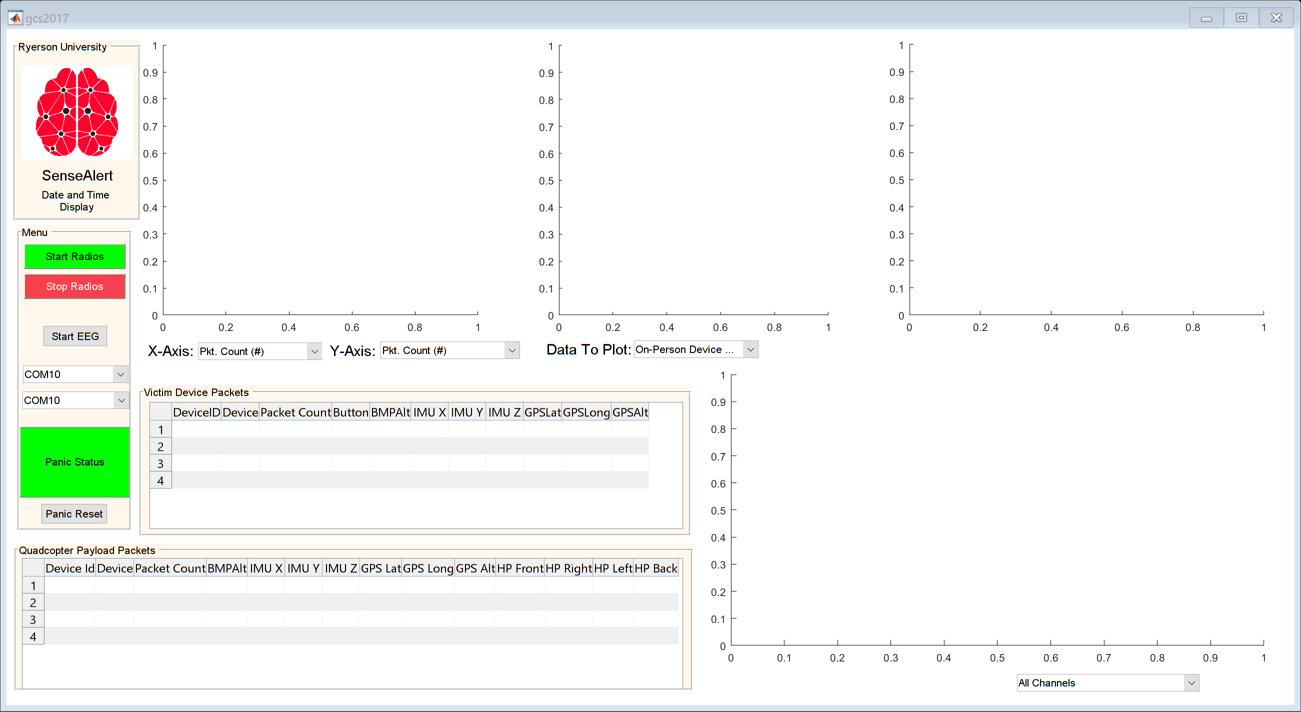
\includegraphics [width=4in]{gcs2017_01.png}



\end{document}
    
